\subsection{Entropy-based search}
\begin{frame}
\frametitle{Entropy-based search\cite{panigrahy2006entropy}}
\small
\begin{itemize}
	\item Use one or a few hash table and hash several randomly chosen points in the neighborhood to reduce time and space complexity
	\vspace{2ex}
	\item  \textbf{Construction of hash table}: pick $k=\frac{\log n}{\log (1/g)}$ random hash functions $h_1, h_2, ..., h_k$. For each point $p$ in the database compute $H(p)=(h_1(p), h_2(p), ..., h_k(p))$ (\alert{after random rotations and shifts for each hash function}) and store $p$ in a table at location $H(p)$. \textit{polylogn} is used to construct hash tables.
	\vspace{2ex}
	\item \textbf{Search}: Given $q$ and $r$, pick $O(n^\rho)$ random points $v$ from $B(q, r)$, where $\rho=\frac{M}{\log(1/g)}$, and search in the buckets $H(v)$.
\end{itemize}
\end{frame}
\subsection{Adaptative LSH}
\begin{frame}
\frametitle{Adaptative LSH\cite{jegou2008query}}
\small
\begin{itemize}
	\item Based on the idea that the relevance of the hash function used in LSH are the lower the better
	\vspace{2ex}
	\item $D_8$ lattice is the set of points of $Z^8$ whose sum is even, e.g. $(1,1,1,1,1,1,1,1)\in D_8$
	\vspace{2ex}
	\item $E_8=D_8\cup (D_8+\frac{1}{2})$
	\vspace{2ex}
	\item $h_i(x)=E_8(\frac{x_{i,8}-b_i}{w})$
\end{itemize}
\end{frame}
\subsection{LSH Forest}

\begin{frame}
\small
	\frametitle{Basic Idea of LSH Forest\cite{bawa2005lsh}}
	\begin{itemize}
		\item $B+$ tree is always accurate
		\vspace{2ex}
		\item Variance number of hash functions for different queries
		\vspace{2ex}
		\item Efficient implementation for main memory and Disk
	\end{itemize}
\begin{figure}
	\begin{center}
		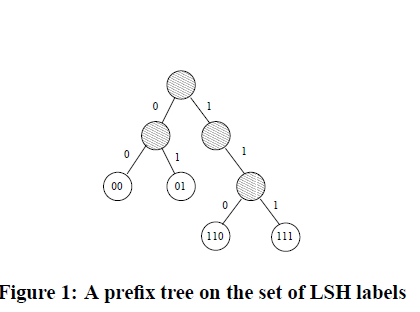
\includegraphics[width=2in]{figures/forest.png}
	\end{center}
\end{figure}
\end{frame}
\begin{frame}
\frametitle{Algorithm for Query}
\begin{figure}
	\begin{center}
		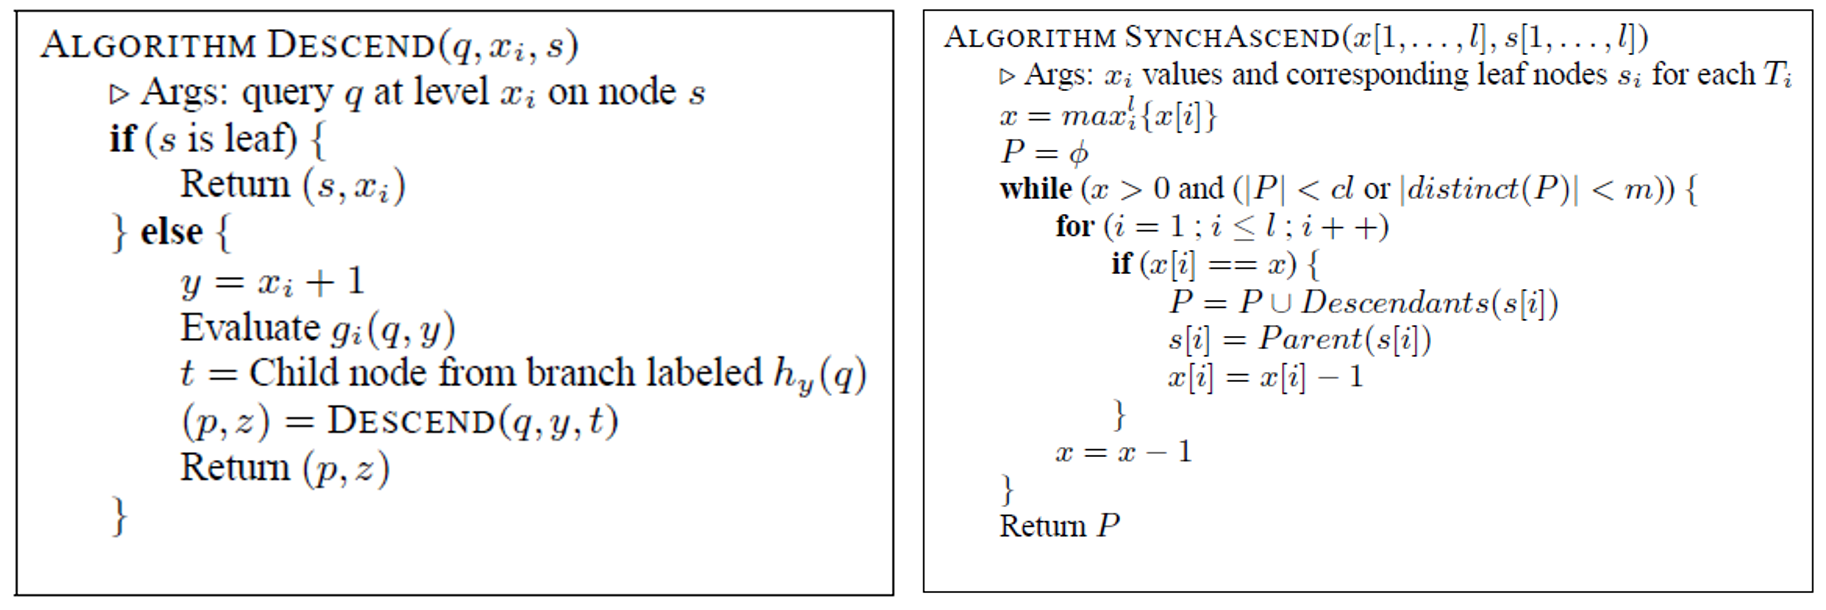
\includegraphics[width=4in]{figures/alg.png}
	\end{center}
\end{figure}
\end{frame}